
%% bare_conf.tex
%% V1.4b
%% 2015/08/26
%% by Michael Shell
%% See:
%% http://www.michaelshell.org/
%% for current contact information.
%%
%% This is a skeleton file demonstrating the use of IEEEtran.cls
%% (requires IEEEtran.cls version 1.8b or later) with an IEEE
%% conference paper.
%%
%% Support sites:
%% http://www.michaelshell.org/tex/ieeetran/
%% http://www.ctan.org/pkg/ieeetran
%% and
%% http://www.ieee.org/

%%*************************************************************************
%% Legal Notice:
%% This code is offered as-is without any warranty either expressed or
%% implied; without even the implied warranty of MERCHANTABILITY or
%% FITNESS FOR A PARTICULAR PURPOSE! 
%% User assumes all risk.
%% In no event shall the IEEE or any contributor to this code be liable for
%% any damages or losses, including, but not limited to, incidental,
%% consequential, or any other damages, resulting from the use or misuse
%% of any information contained here.
%%
%% All comments are the opinions of their respective authors and are not
%% necessarily endorsed by the IEEE.
%%
%% This work is distributed under the LaTeX Project Public License (LPPL)
%% ( http://www.latex-project.org/ ) version 1.3, and may be freely used,
%% distributed and modified. A copy of the LPPL, version 1.3, is included
%% in the base LaTeX documentation of all distributions of LaTeX released
%% 2003/12/01 or later.
%% Retain all contribution notices and credits.
%% ** Modified files should be clearly indicated as such, including  **
%% ** renaming them and changing author support contact information. **
%%*************************************************************************


% *** Authors should verify (and, if needed, correct) their LaTeX system  ***
% *** with the testflow diagnostic prior to trusting their LaTeX platform ***
% *** with production work. The IEEE's font choices and paper sizes can   ***
% *** trigger bugs that do not appear when using other class files.       ***                          ***
% The testflow support page is at:
% http://www.michaelshell.org/tex/testflow/



\documentclass[conference]{IEEEtran}
% Some Computer Society conferences also require the compsoc mode option,
% but others use the standard conference format.
%
% If IEEEtran.cls has not been installed into the LaTeX system files,
% manually specify the path to it like:
% \documentclass[conference]{../sty/IEEEtran}





% Some very useful LaTeX packages include:
% (uncomment the ones you want to load)


% *** MISC UTILITY PACKAGES ***
%
%\usepackage{ifpdf}
% Heiko Oberdiek's ifpdf.sty is very useful if you need conditional
% compilation based on whether the output is pdf or dvi.
% usage:
% \ifpdf
%   % pdf code
% \else
%   % dvi code
% \fi
% The latest version of ifpdf.sty can be obtained from:
% http://www.ctan.org/pkg/ifpdf
% Also, note that IEEEtran.cls V1.7 and later provides a builtin
% \ifCLASSINFOpdf conditional that works the same way.
% When switching from latex to pdflatex and vice-versa, the compiler may
% have to be run twice to clear warning/error messages.





\usepackage{listings}
% *** CITATION PACKAGES ***
%
\usepackage{cite}
% cite.sty was written by Donald Arseneau
% V1.6 and later of IEEEtran pre-defines the format of the cite.sty package
% \cite{} output to follow that of the IEEE. Loading the cite package will
% result in citation numbers being automatically sorted and properly
% "compressed/ranged". e.g., [1], [9], [2], [7], [5], [6] without using
% cite.sty will become [1], [2], [5]--[7], [9] using cite.sty. cite.sty's
% \cite will automatically add leading space, if needed. Use cite.sty's
% noadjust option (cite.sty V3.8 and later) if you want to turn this off
% such as if a citation ever needs to be enclosed in parenthesis.
% cite.sty is already installed on most LaTeX systems. Be sure and use
% version 5.0 (2009-03-20) and later if using hyperref.sty.
% The latest version can be obtained at:
% http://www.ctan.org/pkg/cite
% The documentation is contained in the cite.sty file itself.






% *** GRAPHICS RELATED PACKAGES ***
%
\ifCLASSINFOpdf
\usepackage[pdftex]{graphicx}
  % declare the path(s) where your graphic files are
  % \graphicspath{{../pdf/}{../jpeg/}}
  % and their extensions so you won't have to specify these with
  % every instance of \includegraphics
  % \DeclareGraphicsExtensions{.pdf,.jpeg,.png}
\else
  % or other class option (dvipsone, dvipdf, if not using dvips). graphicx
  % will default to the driver specified in the system graphics.cfg if no
  % driver is specified.
  % \usepackage[dvips]{graphicx}
  % declare the path(s) where your graphic files are
  % \graphicspath{{../eps/}}
  % and their extensions so you won't have to specify these with
  % every instance of \includegraphics
  % \DeclareGraphicsExtensions{.eps}
\fi
% graphicx was written by David Carlisle and Sebastian Rahtz. It is
% required if you want graphics, photos, etc. graphicx.sty is already
% installed on most LaTeX systems. The latest version and documentation
% can be obtained at: 
% http://www.ctan.org/pkg/graphicx
% Another good source of documentation is "Using Imported Graphics in
% LaTeX2e" by Keith Reckdahl which can be found at:
% http://www.ctan.org/pkg/epslatex
%
% latex, and pdflatex in dvi mode, support graphics in encapsulated
% postscript (.eps) format. pdflatex in pdf mode supports graphics
% in .pdf, .jpeg, .png and .mps (metapost) formats. Users should ensure
% that all non-photo figures use a vector format (.eps, .pdf, .mps) and
% not a bitmapped formats (.jpeg, .png). The IEEE frowns on bitmapped formats
% which can result in "jaggedy"/blurry rendering of lines and letters as
% well as large increases in file sizes.
%
% You can find documentation about the pdfTeX application at:
% http://www.tug.org/applications/pdftex





% *** MATH PACKAGES ***
%
%\usepackage{amsmath}
% A popular package from the American Mathematical Society that provides
% many useful and powerful commands for dealing with mathematics.
%
% Note that the amsmath package sets \interdisplaylinepenalty to 10000
% thus preventing page breaks from occurring within multiline equations. Use:
%\interdisplaylinepenalty=2500
% after loading amsmath to restore such page breaks as IEEEtran.cls normally
% does. amsmath.sty is already installed on most LaTeX systems. The latest
% version and documentation can be obtained at:
% http://www.ctan.org/pkg/amsmath





% *** SPECIALIZED LIST PACKAGES ***
%
%\usepackage{algorithmic}
% algorithmic.sty was written by Peter Williams and Rogerio Brito.
% This package provides an algorithmic environment fo describing algorithms.
% You can use the algorithmic environment in-text or within a figure
% environment to provide for a floating algorithm. Do NOT use the algorithm
% floating environment provided by algorithm.sty (by the same authors) or
% algorithm2e.sty (by Christophe Fiorio) as the IEEE does not use dedicated
% algorithm float types and packages that provide these will not provide
% correct IEEE style captions. The latest version and documentation of
% algorithmic.sty can be obtained at:
% http://www.ctan.org/pkg/algorithms
% Also of interest may be the (relatively newer and more customizable)
% algorithmicx.sty package by Szasz Janos:
% http://www.ctan.org/pkg/algorithmicx




% *** ALIGNMENT PACKAGES ***
%
%\usepackage{array}
% Frank Mittelbach's and David Carlisle's array.sty patches and improves
% the standard LaTeX2e array and tabular environments to provide better
% appearance and additional user controls. As the default LaTeX2e table
% generation code is lacking to the point of almost being broken with
% respect to the quality of the end results, all users are strongly
% advised to use an enhanced (at the very least that provided by array.sty)
% set of table tools. array.sty is already installed on most systems. The
% latest version and documentation can be obtained at:
% http://www.ctan.org/pkg/array


% IEEEtran contains the IEEEeqnarray family of commands that can be used to
% generate multiline equations as well as matrices, tables, etc., of high
% quality.




% *** SUBFIGURE PACKAGES ***
%\ifCLASSOPTIONcompsoc
%  \usepackage[caption=false,font=normalsize,labelfont=sf,textfont=sf]{subfig}
%\else
%  \usepackage[caption=false,font=footnotesize]{subfig}
%\fi
% subfig.sty, written by Steven Douglas Cochran, is the modern replacement
% for subfigure.sty, the latter of which is no longer maintained and is
% incompatible with some LaTeX packages including fixltx2e. However,
% subfig.sty requires and automatically loads Axel Sommerfeldt's caption.sty
% which will override IEEEtran.cls' handling of captions and this will result
% in non-IEEE style figure/table captions. To prevent this problem, be sure
% and invoke subfig.sty's "caption=false" package option (available since
% subfig.sty version 1.3, 2005/06/28) as this is will preserve IEEEtran.cls
% handling of captions.
% Note that the Computer Society format requires a larger sans serif font
% than the serif footnote size font used in traditional IEEE formatting
% and thus the need to invoke different subfig.sty package options depending
% on whether compsoc mode has been enabled.
%
% The latest version and documentation of subfig.sty can be obtained at:
% http://www.ctan.org/pkg/subfig




% *** FLOAT PACKAGES ***
%
%\usepackage{fixltx2e}
% fixltx2e, the successor to the earlier fix2col.sty, was written by
% Frank Mittelbach and David Carlisle. This package corrects a few problems
% in the LaTeX2e kernel, the most notable of which is that in current
% LaTeX2e releases, the ordering of single and double column floats is not
% guaranteed to be preserved. Thus, an unpatched LaTeX2e can allow a
% single column figure to be placed prior to an earlier double column
% figure.
% Be aware that LaTeX2e kernels dated 2015 and later have fixltx2e.sty's
% corrections already built into the system in which case a warning will
% be issued if an attempt is made to load fixltx2e.sty as it is no longer
% needed.
% The latest version and documentation can be found at:
% http://www.ctan.org/pkg/fixltx2e


%\usepackage{stfloats}
% stfloats.sty was written by Sigitas Tolusis. This package gives LaTeX2e
% the ability to do double column floats at the bottom of the page as well
% as the top. (e.g., "\begin{figure*}[!b]" is not normally possible in
% LaTeX2e). It also provides a command:
%\fnbelowfloat
% to enable the placement of footnotes below bottom floats (the standard
% LaTeX2e kernel puts them above bottom floats). This is an invasive package
% which rewrites many portions of the LaTeX2e float routines. It may not work
% with other packages that modify the LaTeX2e float routines. The latest
% version and documentation can be obtained at:
% http://www.ctan.org/pkg/stfloats
% Do not use the stfloats baselinefloat ability as the IEEE does not allow
% \baselineskip to stretch. Authors submitting work to the IEEE should note
% that the IEEE rarely uses double column equations and that authors should try
% to avoid such use. Do not be tempted to use the cuted.sty or midfloat.sty
% packages (also by Sigitas Tolusis) as the IEEE does not format its papers in
% such ways.
% Do not attempt to use stfloats with fixltx2e as they are incompatible.
% Instead, use Morten Hogholm'a dblfloatfix which combines the features
% of both fixltx2e and stfloats:
%
% \usepackage{dblfloatfix}
% The latest version can be found at:
% http://www.ctan.org/pkg/dblfloatfix




% *** PDF, URL AND HYPERLINK PACKAGES ***
%
%\usepackage{url}
% url.sty was written by Donald Arseneau. It provides better support for
% handling and breaking URLs. url.sty is already installed on most LaTeX
% systems. The latest version and documentation can be obtained at:
% http://www.ctan.org/pkg/url
% Basically, \url{my_url_here}.




% *** Do not adjust lengths that control margins, column widths, etc. ***
% *** Do not use packages that alter fonts (such as pslatex).         ***
% There should be no need to do such things with IEEEtran.cls V1.6 and later.
% (Unless specifically asked to do so by the journal or conference you plan
% to submit to, of course. )


% correct bad hyphenation here
\hyphenation{op-tical net-works semi-conduc-tor}


\begin{document}
%
% paper title
% Titles are generally capitalized except for words such as a, an, and, as,
% at, but, by, for, in, nor, of, on, or, the, to and up, which are usually
% not capitalized unless they are the first or last word of the title.
% Linebreaks \\ can be used within to get better formatting as desired.
% Do not put math or special symbols in the title.
\title{Baskets Queue c++ Implementation}


% author names and affiliations
% use a multiple column layout for up to three different
% affiliations
\author{\IEEEauthorblockN{Robert Bland}
\IEEEauthorblockA{UCF Computer Science\\
Team \#4}
\and
\IEEEauthorblockN{Jacob Crandall}
\IEEEauthorblockA{UCF Computer Science\\
Team \#4}
\and
\IEEEauthorblockN{Jacob Jiskoot}
\IEEEauthorblockA{UCF Computer Science\\
Team \#4}}

% make the title area
\maketitle

% As a general rule, do not put math, special symbols or citations
% in the abstract
\begin{abstract}
FIFO Queues have been the subject of much research.  They are useful for a number of reasons in concurrent settings.  They can be used to buffer data or quickly create producer / consumer systems.  Because of FIFO Queues wide usage in concurrent (and everyday) programming it is important that effort is made to make them both attainable and preformant.  Today one of the most popular concurrent FIFO Queues is the Michael Scott (MS) queue \cite{ms}.  It is even included in the Java standard library.  The MS queue is fairly preformant and easy to implement.  Its main draw is that the queue provides a lock free algorithm that supports concurrent enqueues and dequeues.  The main issue is that while an enqueue and dequeue can occur conccurently multiple enqueues or multiple dequeues will fail in this case.  \break

The baskests queue \cite{baskets} proposes an implementation that allows for multiple concurrent enqueues or dequeues.  Due to its implementation it is also more portable.  The preformance increase (along with other benefits provided by baskets queue has been proven.  In this paper we will propose a c++ implementation of the baskets queue while discussing its shortcomings, benefits and preformance.  This paper is meant mostly as  discussion of the results and implementation of the baskets queue at a conceptual level.  It is not meant to provide the implementation itself.  Instead we leave it to the reader to use this as a supplementary tool along with our provided source code to understand the baskets queue at an implementational level.
\end{abstract}

% For peerreview papers, this IEEEtran command inserts a page break and
% creates the second title. It will be ignored for other modes.
\IEEEpeerreviewmaketitle



\section{Introduction}
\subsection{Michael-Scott Queue}
The MS queue \cite{ms} provides a lockfree FIFO queue with concurrency at the head and tail.  It provides a straightforward and easy to follow implementation that makes it an easy base for both every day use and for research so it makes sense try to improve on this algorithm.  In the MS queue if two concurrent enqueues (or dequeues) occur then one will succeed or one will fail (or if there are three concurrent enques one will succeed and two will fail, etc.).  The failed operation will back-off and try again later.  

\begin{figure}[!h]
\centering
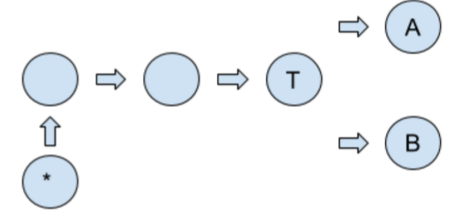
\includegraphics[width=2.5in]{msqueue}
\DeclareGraphicsExtensions.
\caption{Example of concurrent enqueue to an MS queue in a linked list implementation. Assume that A succeeds then B must re-traverse the list and back off before trying to insert again.  In this case it must re-traverse the list as well, further hurting preformance.}
\label{fig_sim}
\end{figure}

This gives the MS queue more difficulty in highly concurrent environments.  The back-off helps this concurrency issue but it introduces new issues.  The back-off scheme can be difficult to deal with for its own reasons as it requires tweaking that is specific to the system running the code.  Even if you find some library implementation if you want optimal preformance you will have to take time to tweak and test parameters.
\subsection{Baskets Queue}
The baskets queue \cite{baskets} is based off of the MS queue but proposes changes to deal with both its concurrency issues and the back-off scheme problem.  The baskets queue can be extended to other queues as well, such as the optimistic FIFO queue \cite{opt}.  However, in this implementation we will be looking at an implementation that is based off of the MS queue in a linked list form.

\begin{figure}[!h]
\centering
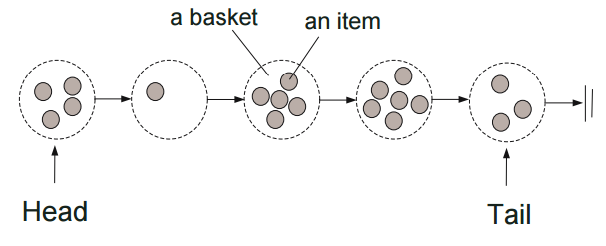
\includegraphics[width=3in]{abstractBasket}
\DeclareGraphicsExtensions.
\caption{Image taken from \cite{baskets}.  This is the abstract baskets queue based on a linked list implementaiton.  Nodes are individual baskets whereas the baskets are just conceptual, not real structures. }
\label{fig_sim}
\end{figure}

The main principal behind the baskets queue presented in \cite{baskets} is that concurrent operations can be re-ordered in any order and still be linearizable.  So for example if we preform two concurent operations \(enqueue(A)\) and \(enqueue(B)\) then the output when dequeuing could be \(A\rightarrow B\) or \(B\rightarrow A\) and still be considered correct.  We may retroactively set the linearization points and thus have a correct implementation regardless of actual outcome of the dequeues.
\break
In the case of no concurrent enqueues or dequeues the baskets queue based on the MS queue behaves exactly like the MS queue.  It is when conflicts occur that an item is inserted into a basket and the baskets are considered a kind of "back-off" scheme.  It is in these concurrent situations that the baskets come into play.
Each item that is being inserted into the basket will have happened concurrently, meaning that it failed on the compare and swap operation that tried to move the either the head or tail of the queue.  

\begin{figure*}[!tp]
\centering
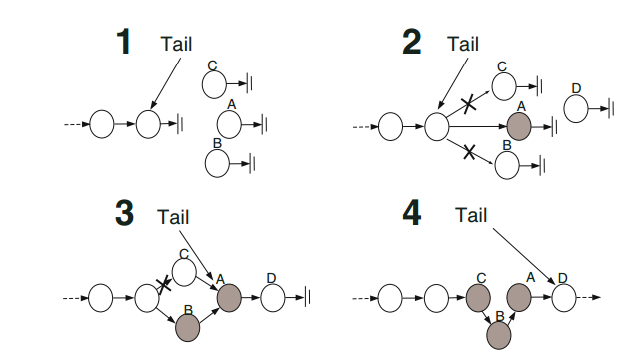
\includegraphics[width=5in]{basketsInsert}
\DeclareGraphicsExtensions.
\caption{Image taken from \cite{baskets}.  This is the abstract baskets queue based on a linked list implementaiton.  Nodes are individual baskets whereas the baskets are just conceptual, not real structures. }
\label{fig_sim}
\end{figure*}

In this case (like the MS queue) one item will succeed but the rest that failed will insert into the queue in any order.  The major benefit is that the first successful enqueue becomes the new queue tail while the other inserts get linked "before" this new tail.  Because of this enqueues can continue to happen past that new tail making it so that \textbf{concurrent operations can happen between different baskets}.  However, concurrent operations still may not occur per basket.  In \cite{baskets} they show that in many cases there will only be around three items per basket (even with high concurrency) which makes it so that a back-off scheme is not necessary.  If there is a highly highly concurrent environment though it may be of interest to implement a back-off scheme within the basket insert but otherwise the problem is minimized and less of concern. \break

The dequeue of the baskets queue is more or less the same as that in the MS queue proposed in \cite{ms}.  That is when a node to remove is found then the queue will preform a compare and swap on the head, if there are issues finding some non-deleted node between head and tail then some action will be taken to correct it (often times just updating head values and trying again) or the queue may have been empty, in which case we simply return NULL.  It is important to note that while enqueues will always succeed (sit in the while loop until they enqueue) that a dequeue will immediately return NULL if the queue is found to be empty, it will not spin and wait for a value to be inserted.\break

The baskets queue in \cite{baskets} adds some auxilary features to the original MS queue presented in \cite{ms}.  One of these is the ability to logically delete nodes.  This is added by editing the pointer itself to store extra information.  Furthermore along with the "deleted" bit a counter is also implemented to avoid the ABA problem.  The use of logically deleted nodes is a popular method that allows us to essentially save hard work for later and do it all at once.  That is exactly what is done in this case.  When a chain of length X or more is found while removing nodes (a thread counts while traversing) then a chain will be physically deleted.  This is done by resetting the tail (in an "if compare and swap" so that only one function will enter the free chain method) which cuts off all public access to this chain.  The thread inside this free chain method is then free to reclaim nodes as it can.\break

\section{Implementation}
Our implementation is based heavily on the pseudo-code provided in \cite{baskets}.  For the most part this pseudo-code, our code and the concepts presented may be studied to gather a very detailed understanding of how the baskets queue operates.\break
If directly running the provided code the program takes the following arguments:
\begin{itemize}
  \item Arg1 : Number of threads : How many threads will be preforming tasks
  \item Arg2 : Number of jobs (Enqueues \& Dequeues)
  \item Arg3 : Percentage of enqueues (the rest will be dequeues)
  \item Arg4 : Number of pre-populated nodes : 0 - Inf
\end{itemize}
After compiling with the provided make file the program may be run as an example
\begin{lstlisting}
./main 4 500 .6 0
\end{lstlisting}
This will create 4 threads that together will execute 500 enqueue or dequeues, 60\% of which will be enqueues and 40\% of will be dequeues.  The "number of pre-populated nodes" argument will be described below.

\subsection{Supporting Implementation}
We define a sort of "harness" that we use to give an example implementation of the baskets queue.  There are two main parts of this.  First is the sections that support simply running the baskets queue, that is a system for actually preforming enqueues and dequeues.  This section may be skipped if the reader wishes as it is mostly about how we tested and utilized the queue itself.  There are some concepts that apply towards concurrent programming here though that may still be of interest.  Secondly we have sections of code that support the baskets queue itself.  These are sections that are abstracted away by the pseudo-code in \cite{baskets}.  These include things like pointer manipulation for tags and counting.\break

\subsubsection{Preforming Enqueues and Dequeues}
The objects we are inserting are based around a specialized node class.  If looking into using the provided code in a similar implementation it would be simple to retain all specialized node related work and simply change the payload of the nodes.  For our case we are utilizing ints, this was an arbitrary decision and any sort of payload could be used here.  We first take some pre-cautions to prepare our threads for a multi-threaded environment.  This means that we want to seed our random jobs (percentage of enqueues / dequeues) before spinning up threads.  This is because the provided c++ random implementation is not gauranteed to be thread safe.  Each thread will then continually take jobs from this seeded jobs array until it is empty.  \break
Similarly to how we seed randoms we also seed nodes.  That is, each thread is provided a local list of nodes.  When it enqueues it pulls a new node address from this list and inserts it into the queue.  When dequeing we return a pointer to such a node, the thread will reattach this pointer to its local node list.  In this way we avoid ever have to allocate new memory in a concurrent environment.  This is what the previous "number of pre-populated nodes" argument was for.  We left it up to the user to determine a safe number of nodes to pre-allocate per thread.  For example if preforming 99\% dequeues then each thread may only need a small number of pre-allocated nodes but technically still with 99\% dequeues we could have all enqueues.  (We do not gaurantee a certain number of enqueue / dequeues as jobs are seeded randomly with bias).  So the user may want to be safe and give each thread the same number of nodes as number of jobs.  As a side note we did find some unreliable information that suggests that this may not be necessary.  It was suggested that if the pthreads library is linked (which it is, via our make file) then instead of the standard malloc / new memory allocators a thread safe malloc is loaded.  It is worth noting however that this thread safe malloc could still have locks, hurting the runtime preformance.  For those multiple reasons we leave it up to the user to determine how they would like to handle node pre-allocation.  In our implementation we do not make an effort to clean the nodes either, this could be simply done once work is determined to be done however.\break
We do make one intrusive change to the basket queue in order to support this pre-allocated node behavior.  In the original baskets queue dequeue method pseudo-code provided in \cite{baskets} they provide a generalized "recycle node" function.  This is meant to do exactly as we describe above.  That is it makes some node pointer available to be re-used.  The implementation will still work if this is re-worked to be a more widely available methodology.
\subsubsection{Baskets Specific Auxilary Work}
There is work outside of what is provided within the contents of the paper that this implementation is based off of \cite{baskets}.  Namely, the baskets paper \cite{baskets} does not provides simply pseudo-code and assumes available implementations for certain tasks.  The largest of these tasks is the creation data structures that can be atomically swapped that include pointers, integers and a boolean.  The baskets queue relies heavily on the ability to preform atomic compare and swap operations on multiple pieces of data.  It is required to be able to atomically swap a pointer, a reference counter (how many times the node has been touched) and the logical deletion flag that was mentioned earlier.  This is not a behavior that is native to c++ so we must implement it manually.  From our classes we learned that not all bits of a pointer are utilized.  So we may utilize those ending bits without changing the valid values of the pointer.  We do this by preforming bitwise operations to save values as needed.\break
\subsection{Baskets Implementation}
TODO: Talk about how we dont implement backoffs and other specifics to our implementation, could just walk through what our baskets.cpp does here mostly
\subsection{Personal Experiences}
One of the benefits of the baskets queue is that it is more portable than some other queues, especially those that heavily rely on back-off schemes.  For that reason we were reluctant to implement the bit stealing operations as they are not portable.  This is because the number of bits which must be stolen is different per system.  To satisfy this portability requirement we tried to build in constants for any bit stealing operations we utilize.  In the end we believe this implementation is still more portable than altering back-off scheme parameters which may require further testing; although we would like this implementation to be more portable if possible.  For our specific machine implementation (Ubuntu 16.04 x86\_64 architecture) the number of valid bits for stealing was found to be four.  Unfortunately this means that after storing the logical deletion bit we only have three bits to store a reference counter.  This introduces issues if we need four bits to store how many times a node has been referenced (which probably will happen often in any meaningful implementation).  This is the biggest issue with our implementation, it does not completely eliminate the ABA problem but simply avoids it.  The tags will often times not line up with references if an ABA problem arises but it is still possible.  This could be fixed if we utilized a Compare and Swap two as our professor suggested in conversation.  This would allow us to compare and swap with our pointer (which could still use the stolen logical deletion bit) and some unsigned int in one atomic step.  However, we were unable to find any such working implementation for c++.
\textbf{TODO continue working on difficulties, etc.}
\section{Benchmarks \& Experimentation}
\subsection{The Experiments}
Talk about machine we ran the tests on and what we benchmarked against
\subsection{Results}


% An example of a double column floating figure using two subfigures.
% (The subfig.sty package must be loaded for this to work.)
% The subfigure \label commands are set within each subfloat command,
% and the \label for the overall figure must come after \caption.
% \hfil is used as a separator to get equal spacing.
% Watch out that the combined width of all the subfigures on a 
% line do not exceed the text width or a line break will occur.
%
%\begin{figure*}[!t]
%\centering
%\subfloat[Case I]{\includegraphics[width=2.5in]{box}%
%\label{fig_first_case}}
%\hfil
%\subfloat[Case II]{\includegraphics[width=2.5in]{box}%
%\label{fig_second_case}}
%\caption{Simulation results for the network.}
%\label{fig_sim}
%\end{figure*}
%
% Note that often IEEE papers with subfigures do not employ subfigure
% captions (using the optional argument to \subfloat[]), but instead will
% reference/describe all of them (a), (b), etc., within the main caption.
% Be aware that for subfig.sty to generate the (a), (b), etc., subfigure
% labels, the optional argument to \subfloat must be present. If a
% subcaption is not desired, just leave its contents blank,
% e.g., \subfloat[].


% An example of a floating table. Note that, for IEEE style tables, the
% \caption command should come BEFORE the table and, given that table
% captions serve much like titles, are usually capitalized except for words
% such as a, an, and, as, at, but, by, for, in, nor, of, on, or, the, to
% and up, which are usually not capitalized unless they are the first or
% last word of the caption. Table text will default to \footnotesize as
% the IEEE normally uses this smaller font for tables.
% The \label must come after \caption as always.
%
%\begin{table}[!t]
%% increase table row spacing, adjust to taste
%\renewcommand{\arraystretch}{1.3}
% if using array.sty, it might be a good idea to tweak the value of
% \extrarowheight as needed to properly center the text within the cells
%\caption{An Example of a Table}
%\label{table_example}
%\centering
%% Some packages, such as MDW tools, offer better commands for making tables
%% than the plain LaTeX2e tabular which is used here.
%\begin{tabular}{|c||c|}
%\hline
%One & Two\\
%\hline
%Three & Four\\
%\hline
%\end{tabular}
%\end{table}


% Note that the IEEE does not put floats in the very first column
% - or typically anywhere on the first page for that matter. Also,
% in-text middle ("here") positioning is typically not used, but it
% is allowed and encouraged for Computer Society conferences (but
% not Computer Society journals). Most IEEE journals/conferences use
% top floats exclusively. 
% Note that, LaTeX2e, unlike IEEE journals/conferences, places
% footnotes above bottom floats. This can be corrected via the
% \fnbelowfloat command of the stfloats package.
% use section* for acknowledgment
\section*{Acknowledgment}
We would like to thank professor Damian Dechev for teaching and some consultation concerning this project.
\section{Conclusion}
The conclusion goes here.




% conference papers do not normally have an appendix


% use section* for acknowledgment
%\section*{Acknowledgment}


%The authors would like to thank...





% trigger a \newpage just before the given reference
% number - used to balance the columns on the last page
% adjust value as needed - may need to be readjusted if
% the document is modified later
%\IEEEtriggeratref{8}
% The "triggered" command can be changed if desired:
%\IEEEtriggercmd{\enlargethispage{-5in}}

% references section

% can use a bibliography generated by BibTeX as a .bbl file
% BibTeX documentation can be easily obtained at:
% http://mirror.ctan.org/biblio/bibtex/contrib/doc/
% The IEEEtran BibTeX style support page is at:
% http://www.michaelshell.org/tex/ieeetran/bibtex/
\bibliographystyle{IEEEtran}
% argument is your BibTeX string definitions and bibliography database(s)
%\bibliography{bare_conf}
\bibliography{bare_conf}

% that's all folks
\end{document}

